\documentclass[11pt]{article}
\usepackage[a4paper,margin=1in]{geometry}
\usepackage{amsmath,amssymb,amsthm,mathtools}
\usepackage{graphicx}
\usepackage[section]{placeins}
\usepackage{hyperref}
\usepackage{needspace}

\title{Perfect Closure Is Quaternionic: The Riemann Critical Line as a Complex Shadow}
\author{John Van Geem / RQM Technologies}
\date{April 2026}

\begin{document}
\maketitle

\begin{abstract}
This paper provides the geometry layer of the series. The complex critical-line variable $1/2+it$ is lifted to quaternionic slices
\[
q_{\mathbf u}(t)=\frac12+\mathbf u t,\qquad \mathbf u^2=-1.
\]
The classical line is the special slice $\mathbf u=i$. We carefully separate affine slice location from unit-phase closure $Q=e^{\mathbf u\phi}$, and we record the six-step cadence $Q^3=-1$, $Q^6=1$ when $\operatorname{Re}(Q)=1/2$. That cadence is geometric intuition only. The paper does not claim a quaternionic proof of RH.
\end{abstract}

\Needspace{10\baselineskip}
\section*{Reader Guide}
Paper 2 answers: \textbf{why does the complex trace naturally sit inside quaternionic closure geometry?}

The intent is modest and structural. We are not replacing complex analysis. We are showing that the critical-line object from Paper 1 can be viewed as one member of a broader slice family. This lets later papers discuss a shared parameter $t_n$ across complex, operator, and mass-shell language.

\Needspace{10\baselineskip}
\section{Quaternionic slices and critical hyperslice}
Let $\mathbf u$ be a unit imaginary quaternion with $\mathbf u^2=-1$. Define
\[
\mathbb C_{\mathbf u}=\{a+\mathbf u b:\;a,b\in\mathbb R\}.
\]
This equation says that every choice of orientation axis $\mathbf u$ generates a copy of complex numbers inside $\mathbb H$.

Now define the quaternionic critical hyperslice
\[
\Sigma_{1/2}=\{q\in\mathbb H:\operatorname{Re}(q)=1/2\},
\]
with affine slice family
\[
q_{\mathbf u}(t)=\frac12+\mathbf u t.
\]
The first formula defines a three-dimensional real hypersurface in quaternion space. The second formula selects a one-dimensional trajectory inside that surface for a fixed $\mathbf u$.

For $\mathbf u=i$, this becomes exactly the classical critical line $1/2+it$. So the complex line is not discarded; it is recovered as a distinguished slice.

\begin{figure}[htbp]
  \centering
  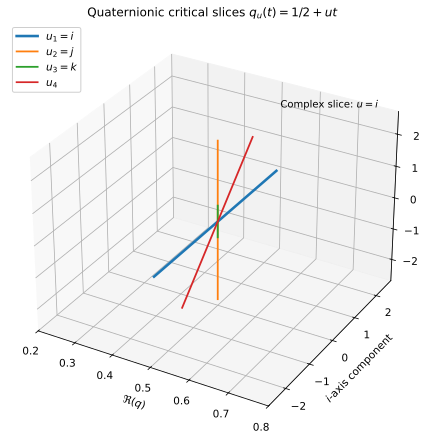
\includegraphics[width=0.80\textwidth]{../assets/figures/quaternionic-critical-slices.svg}
  \caption{The classical critical line $s=1/2+it$ is highlighted as one slice ($\mathbf u=i$) inside the quaternionic family $q_{\mathbf u}(t)=1/2+\mathbf u t$. This supports the slice-lift viewpoint and does not prove any zeta zero statement by itself.}
\end{figure}

\Needspace{10\baselineskip}
\section{Affine slice versus unit phase}
Two equations appear similar but represent different structures:
\begin{itemize}
  \item Affine slice location:
  \[
  q=\frac12+\mathbf u t.
  \]
  \item Unit-phase motion:
  \[
  Q=e^{\mathbf u\phi}=\cos\phi+\mathbf u\sin\phi.
  \]
\end{itemize}

The affine variable $q$ tracks position in a translated linear slice. The unit variable $Q$ tracks rotation on the unit 3-sphere in quaternionic phase. Keeping this distinction explicit prevents mixing additive geometry with multiplicative cadence.

In practical terms, $t$ in $q$ is a coordinate parameter. The angle $\phi$ in $Q$ is a phase parameter. They can be related in models, but they are not automatically identical objects.

\Needspace{10\baselineskip}
\section{Six-step cadence as geometric intuition}
If $\operatorname{Re}(Q)=1/2$, then from
\[
Q=\cos\phi+\mathbf u\sin\phi
\]
we get
\[
\cos\phi=\frac12.
\]
Hence $\phi=\pi/3$ modulo $2\pi$, so for $Q=e^{\mathbf u\pi/3}$, powers step by 60-degree increments:
\[
Q^3=e^{\mathbf u\pi}=-1,\qquad Q^6=e^{\mathbf u2\pi}=1.
\]
This is a compact closure cycle: half-turn to $-1$, full turn to identity. It gives geometric intuition for why the real-part value $1/2$ repeatedly appears in closure motifs.

\begin{figure}[htbp]
  \centering
  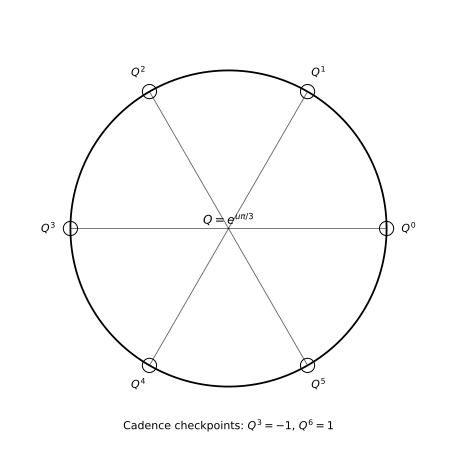
\includegraphics[width=0.56\textwidth]{../assets/figures/six-step-closure-gate.svg}
  \caption{Six-step unit-phase cadence at 60-degree increments for $Q=e^{\mathbf u\pi/3}$, showing $Q^3=-1$ and $Q^6=1$. This cadence is geometric intuition and is not the proof of the zeta-mass bridge.}
\end{figure}

Important caution: this cadence by itself does not produce $\Xi(t_n)=0$. It provides interpretive geometry, while the actual bridge to spectral conditions is formulated with the operator in Paper 4.

\Needspace{10\baselineskip}
\section{Quaternionic lift of the prime phase and residual}
The critical-line prime route from Paper 1,
\[
p^{-(1/2+it)}=p^{-1/2}e^{-it\log p},
\]
lifts slice-wise to
\[
p^{-(1/2+\mathbf u t)}=p^{-1/2}e^{-\mathbf u t\log p}.
\]
The amplitude is unchanged at $p^{-1/2}$; only phase orientation depends on the chosen slice axis $\mathbf u$.

Let
\[
\Xi(t)=\xi\!\left(\frac12+it\right).
\]
A compatible quaternionic slice lift is
\[
\xi_{\mathbb H}(1/2+\mathbf u t)=\operatorname{Re}\Xi(t)+\mathbf u\operatorname{Im}\Xi(t).
\]
This simply packages the same real and imaginary data into the chosen slice plane. The norm identity
\[
\|\xi_{\mathbb H}(1/2+\mathbf u t)\|^2=|\Xi(t)|^2
\]
shows that residual magnitude is slice-consistent.

So the same complex spectral trace data can be read across quaternionic orientation slices, without changing the scalar closure score.

\subsection*{Equation-reading summary for Section 4}
It is useful to read the four equations in this section as a pipeline:
\begin{enumerate}
  \item $p^{-(1/2+it)}=p^{-1/2}e^{-it\log p}$ isolates amplitude and phase on the classical line.
  \item $p^{-(1/2+\mathbf u t)}=p^{-1/2}e^{-\mathbf u t\log p}$ keeps the same amplitude but rotates the phase axis.
  \item $\xi_{\mathbb H}(1/2+\mathbf u t)=\operatorname{Re}\Xi(t)+\mathbf u\operatorname{Im}\Xi(t)$ repackages the same residual components in a slice.
  \item $\|\xi_{\mathbb H}\|^2=|\Xi|^2$ confirms scalar closure magnitude is unchanged by that repackaging.
\end{enumerate}

Seen this way, the lift is conservative: it adds geometric orientation freedom without changing the underlying scalar residual content.

\Needspace{10\baselineskip}
\section{Non-claims and bridge}
\begin{itemize}
  \item No proof of RH.
  \item No claim of a full quaternionic analytic continuation theory.
  \item No mass-shell prediction in this paper.
\end{itemize}

Bridge sentence: Paper 3 defines mass-shell norm language in physical kinematics, and Paper 4 then connects that norm to the same closure eigenvalue $t_n$ used by the zeta trace.

\Needspace{10\baselineskip}
\section*{References}
\begin{enumerate}
  \item W. R. Hamilton, \emph{Elements of Quaternions}, 1866.
  \item S. L. Adler, \emph{Quaternionic Quantum Mechanics and Quantum Fields}, Oxford Univ. Press, 1995.
  \item E. C. Titchmarsh and D. R. Heath-Brown, \emph{The Theory of the Riemann Zeta-Function}, 2nd ed., 1986.
\end{enumerate}

\end{document}
